
It was shown in the chapter \ref{chapter:4} that all examined models of the first reaction stage, i.e. INCL++ \cite{INCLMancusi2014}, UrQMD \cite{UrQMDBASS1998,UrQMDBleicher1999} and GiBUU \cite{GiBUUBuss2012}  are almost equivalent in description of the double differential cross-sections for production of light charged particles (LCP). Among these models, the INCL++  has the technical advantage that it can be easily coupled with the de-excitation models such as ABLA \cite{kelic2009abla07}, GEMINI  \cite{CHARITY1988,Charity2010}, GEM  \cite{FURIHATA2000,Furihata2002} and SMM  \cite{SMMBondorf1995}. Moreover, a hypothesis of  coalescence is included for the formation and  emission of lighter composite  particles (A$<$8) during the first stage of reaction. 

In this chapter, presented are the results of the analysis of $^{136}Xe$+$p$ reaction at energy of 
1 GeV/nucleon \cite{napolitani2007measurement}, confronted with the model predictions for the emission of intermediate mass fragments (IMF)  and heavy target residues.
%with the experimental data.

The present analysis was performed in the framework of the two-step microscopic models. The first step of the reaction was simulated by INCL++ (v5.3), which describes the intranuclear cascade of nucleon-nucleon and pion-nucleon collisions. This process leaves an excited heavy remnant in the equilibrium stage. Later, the de-excitation of the equilibrated heavy remnant  is simulated by 4 different theoretical models  \cite{kelic2009abla07,Furihata2002,Charity2010,SMMBondorf1995}. 

The data studied here cover a very wide range of produced elements, from $Li$ (Z = 3) to $Ba$ (Z = 56). This work is a continuation of the recent study \cite{sharma2017ranking}, where the same reactions were analyzed at lower energy (0.5 GeV/nucleon). At that time, the examined data  \cite{giot2013isotopic} included only heavy reaction products, i.e. nuclei from $Nb$ (Z = 41) to $Ba$ (Z = 56). It was found that all the used theoretical models provided reasonable qualitative agreement with the data, although perfect quantitative agreement was not achieved.
%%%


%\section{$^{136}Xe$ + p at 1GeV/A}
%The present analysis was performed in the frame of the
%two-stage microscopic model. The first step of the process
%was described as intranuclear cascade of nucleon-nucleon
%and pion-nucleon collisions leading to the equilibrated, excited
%remnant nucleus. It was realized by the INCL++
%(version 5.3) model \cite{INCLMancusi2014}. The de-excitation of the equilibrated
%heavy products of the first step of the process
%has been calculated in the frame of four different models:
%ABLA07 \cite{kelic2009abla07}, GEM2 \cite{FURIHATA2000,Furihata2002}, GEMINI++ %\cite{CHARITY1988,Charity2010} and
%SMM \cite{SMMBondorf1995}. The physical assumptions of the models as
%well as the details of their realization may be found in
%the references cited above. The most important
%information is already summarized in chapter \ref{chapter:2}.


\section{Analysis of isotopic cross-sections}

The calculations of the isotopic production cross-sections measured by Napolitani et al. \cite{napolitani2007measurement} for the system $^{136}Xe$+$p$ at 1 GeV per nucleon were performed with default values of the parameters of all the models. Therefore it was possible to judge about the predictive power of the applied models. Results of the calculations are presented in figures \ref{Z0314}, \ref{Z1532} and \ref{Z3356} for light ($2 <$ Z $< 15$), intermediate mass ($14 <$ Z $< 33$) and heavy (32 $<$ Z $<$ 57) reaction products, respectively. The qualitative agreement of the theoretical cross-sections with the data will be discussed below for each range of the products separately. 

It is obvious from the inspection of fig. \ref{Z0314} that the GEM2 model underestimates systematically all the data. Furthermore, the theoretical cross-sections decrease much faster with increasing of the atomic number Z than the data. In result the theoretical cross-sections of GEM2 are negligibly small for Z $>$ 9. 

The isotopic cross-sections predicted by other models do not deviate so significantly from the data. Especially, there is not visible such a systematic underestimation of the data as well as its increase with the atomic number. 
All the models produce bell shaped mass distributions of the isotopic cross-sections similar to the distributions of the experimental cross-sections. However, none of the models reproduces exactly the behaviour of the data. 

Absolute values of the cross-sections predicted by ABLA07 for Z $<$ 9 are smaller than those of the data (with exception of the carbon and oxygen isotopes which seem to be well reproduced). The shape of the mass distributions is reasonably well reproduced for given element with exception of fluorine, where the distribution is shifted towards small masses, and aluminium as well as silicon, where the theoretical distributions are too broad. 

The SMM model systematically under-predicts the cross-sections for heaviest isotopes whereas it overestimates the cross-sections for lightest isotopes (with exception of nitrogen where all the models do not work well).

GEMINI++ seems to produce proper width and position of the cross-section distributions, however, it usually under-predicts values of the cross-sections.

\begin{figure}
    \centering
    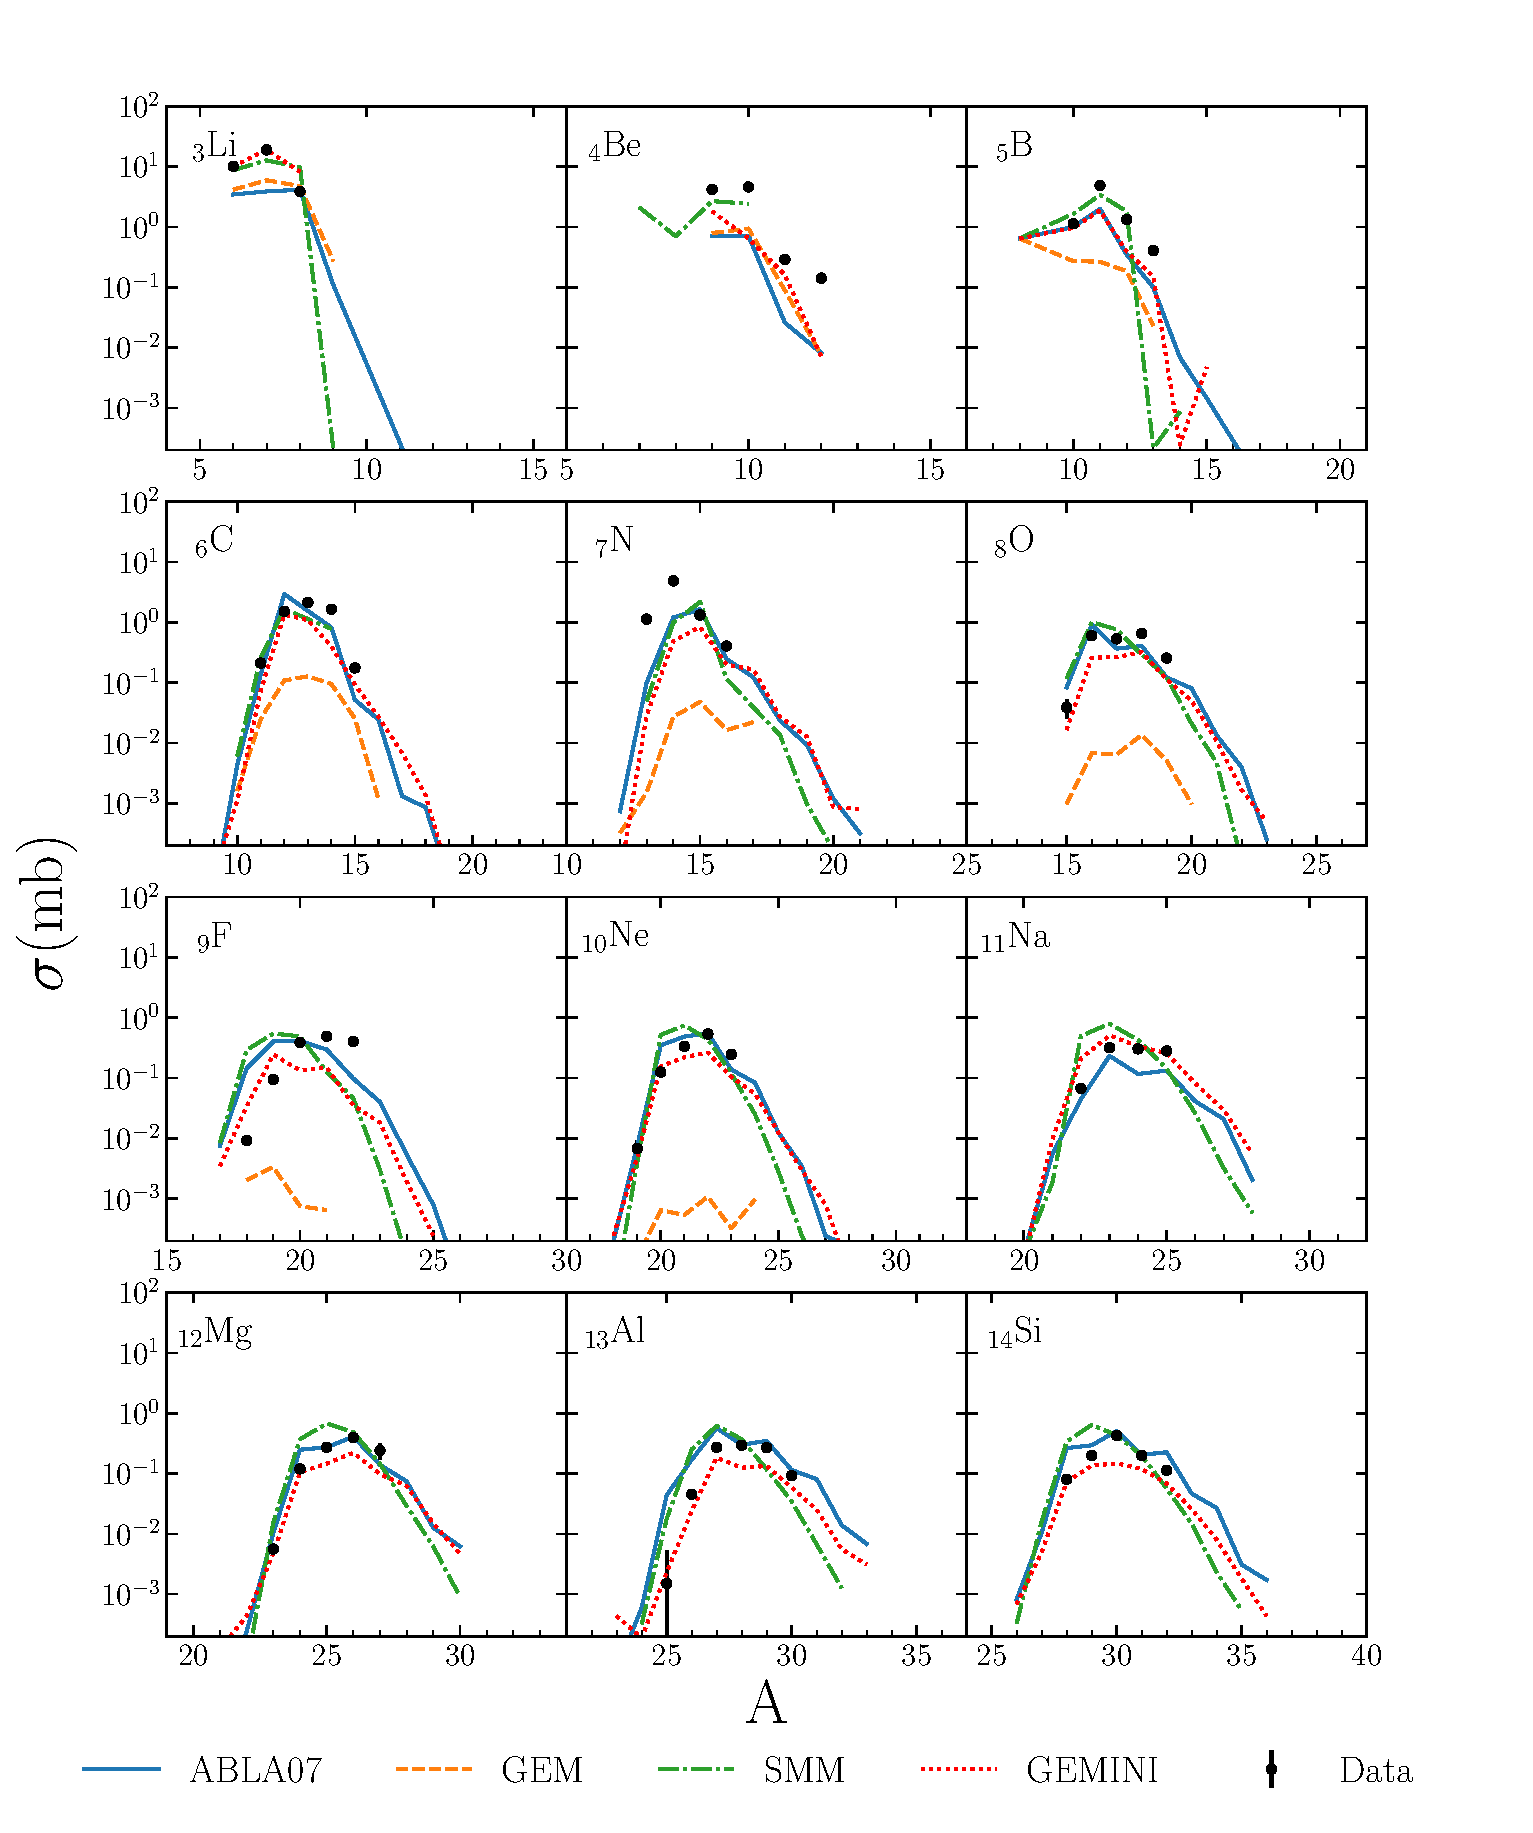
\includegraphics[width=0.9\textwidth]{z0315.eps}
    \caption{Isotopic cross-sections of IMFs with Z = 3–14 from $^{136}Xe$+$p$ collisions at energy T($^{136}Xe$) = 1000 A MeV \cite{napolitani2007measurement} (black dots) together with predictions of the INCL++ (version 5.3) model for the first stage of the reaction coupled to four models of the second stage of reaction: ABLA07 (blue solid line), GEM2 (orange dashed line), GEMINI++ (red dotted line) and SMM (green dashed-dotted line). Note the absence of the theoretical values provided by GEM2 for elements with Z $>$ 10.}
    \label{Z0314}
\end{figure}

The situation is different for elements with 14 $<$ Z $<$ 33. The experimental and theoretical mass distributions of the isotopic cross-sections are presented for these elements in fig. \ref{Z1532}. As can be seen there the GEM2 model does not produce any elements with Z $<$ 30 ($Zn$). Starting from $Zn$ the theoretical cross-sections evaluated with GEM2 appear to be non-negligible but they are more than one order of magnitude smaller than the experimental ones. Thus, the GEM2 cross-sections for the discussed range of elements are completely unrealistic. 

Other models predict the cross-sections which are of the same order of magnitude as the data and, furthermore, the shapes of the mass distributions of the theoretical cross-sections are similar to the shapes of experimental distributions. Nevertheless the systematic deviations of the theoretical cross-sections from the data are observed. 

The mass distributions produced by ABLA07 are too broad in the comparison to the experimental ones. This always leads to the overestimation of the isotopic cross-sections for all isotopes with mass larger than the most populated one and   frequently also for isotopes with the smallest masses. 

The opposite situation is observed for the cross-sections predicted by the SMM model. In this case the cross-sections for isotopes with the smallest mass are systematically overestimated whereas those for the largest masses are systematically underestimated. Thus, in spite of the similarity of the shape of the mass dependence produced by the SMM model and
that observed in the experiment, the absolute values of the cross-sections are systematically overestimated or underestimated by the model. 

Position of the maximum of the mass distribution of the isotopic cross-sections as well as its width is in most cases well reproduced by GEMINI++, however, this model systematically under-predicts the absolute values of the cross-sections. This is most pronounced in the neighbourhood of the maxima of the distributions.

\begin{figure}
    \centering
    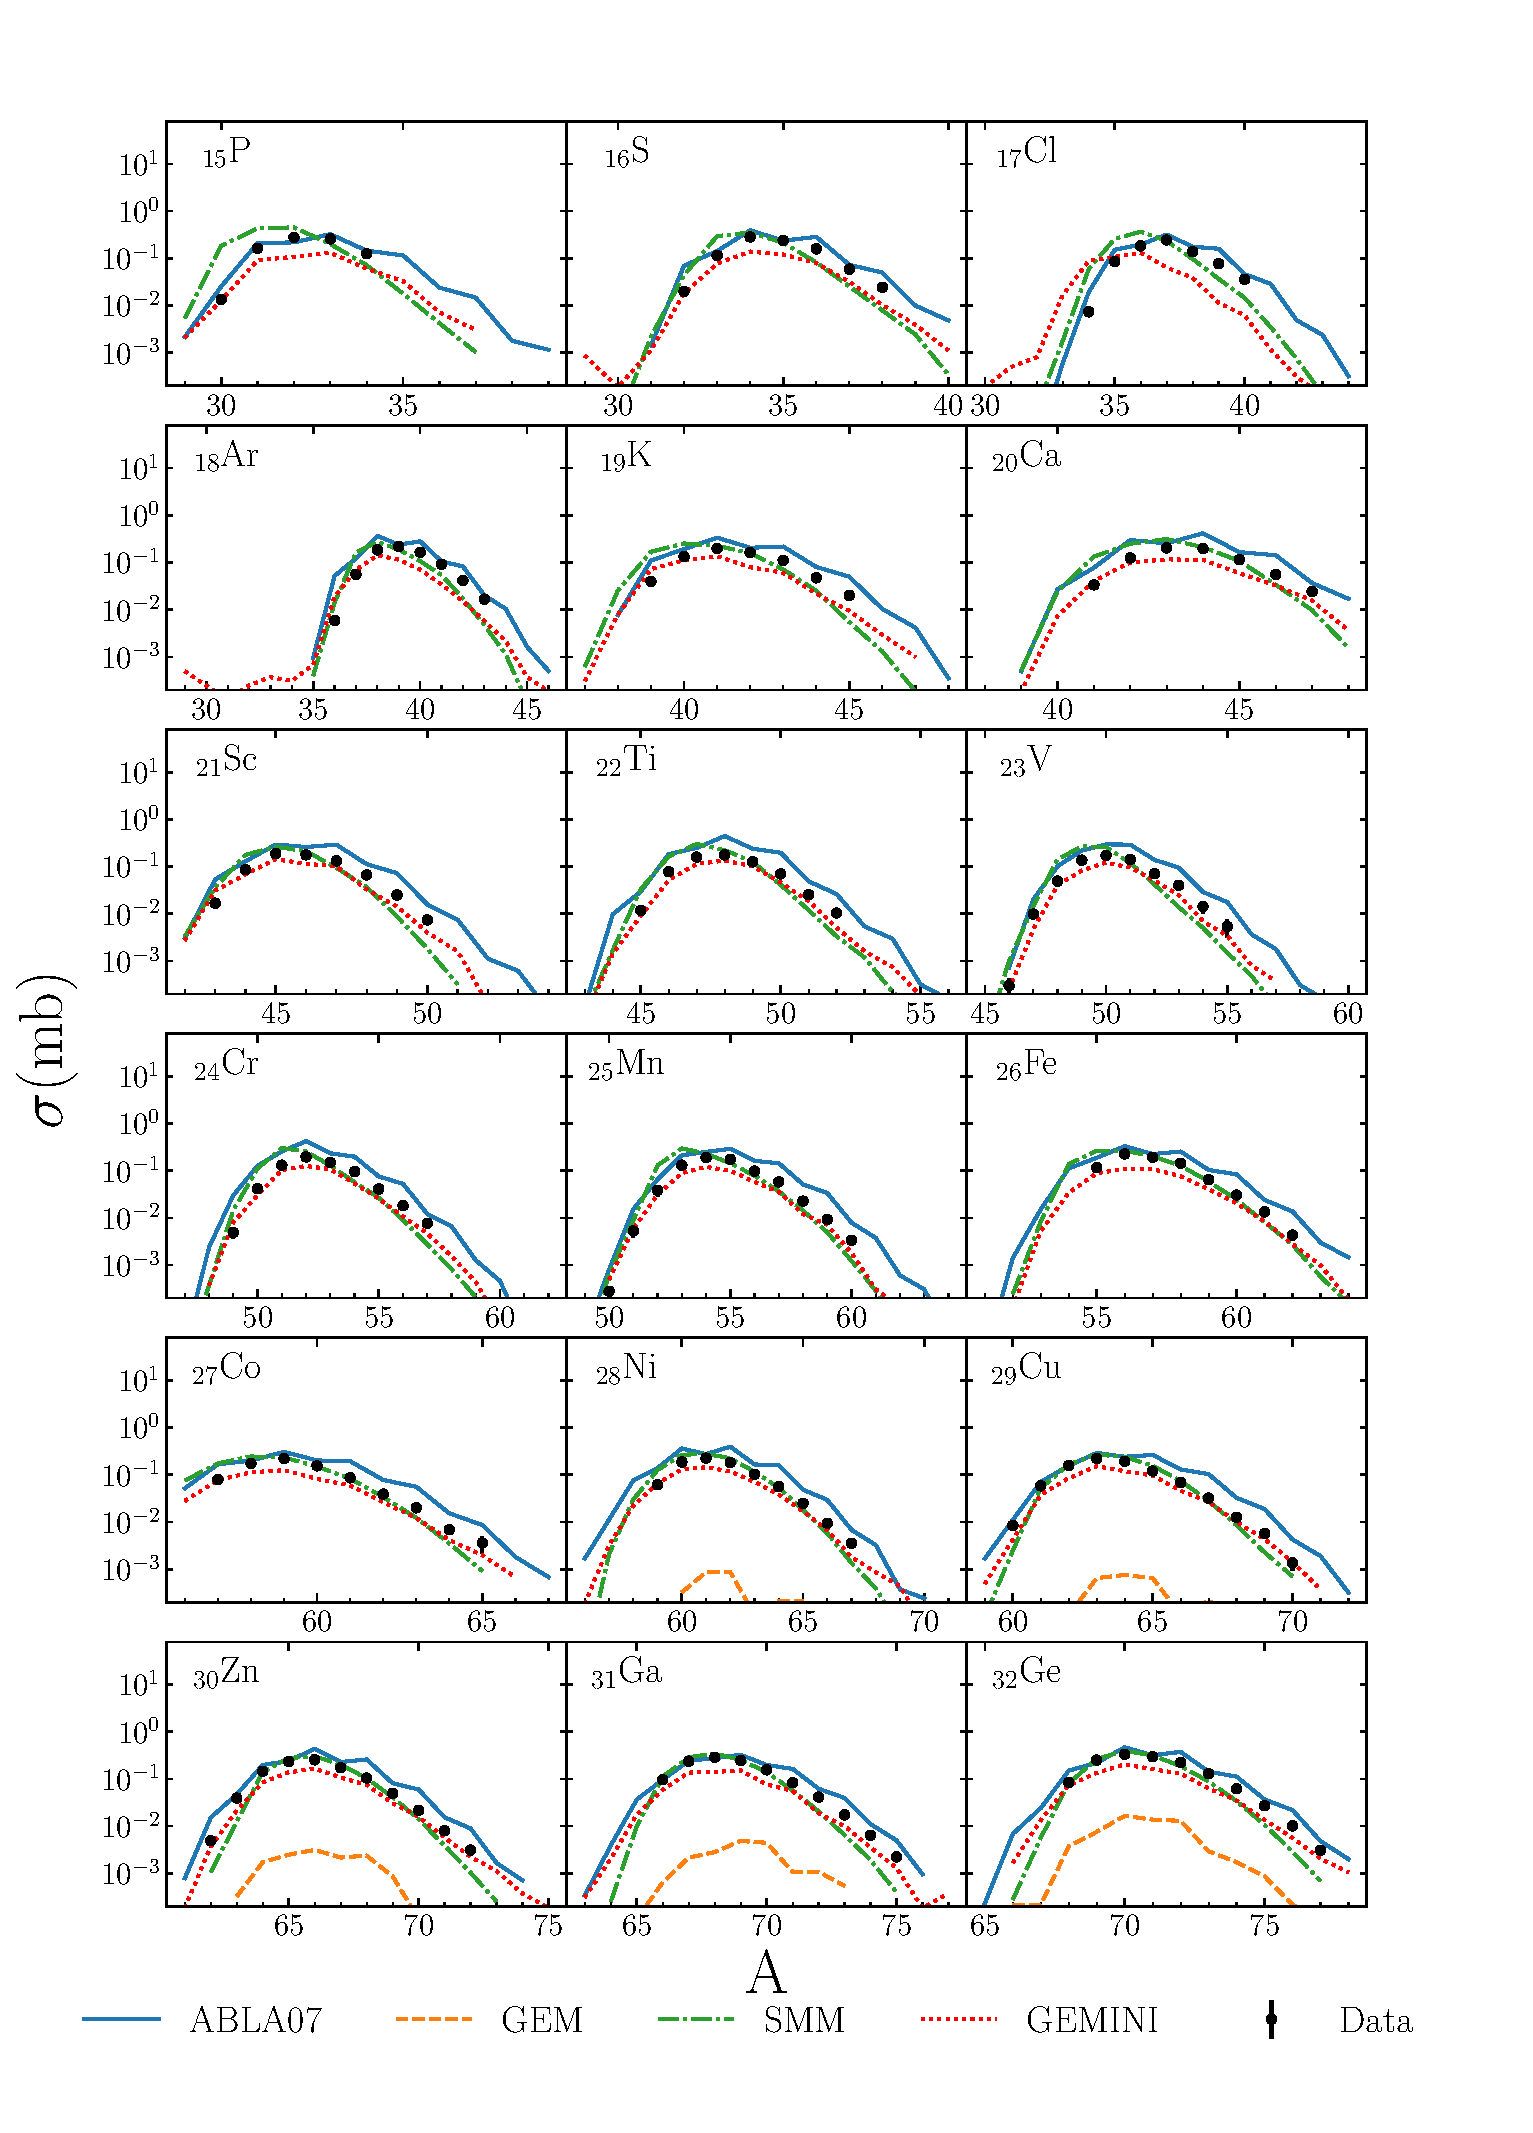
\includegraphics[width=0.93\textwidth]{z1532.eps}
    \caption{The same as in fig. \ref{Z0314}, but for Z = 15–32. Note the absence of the theoretical values provided by GEM2 for elements with Z $<$ 28.}
    \label{Z1532}
\end{figure}
\begin{figure}
    \centering
    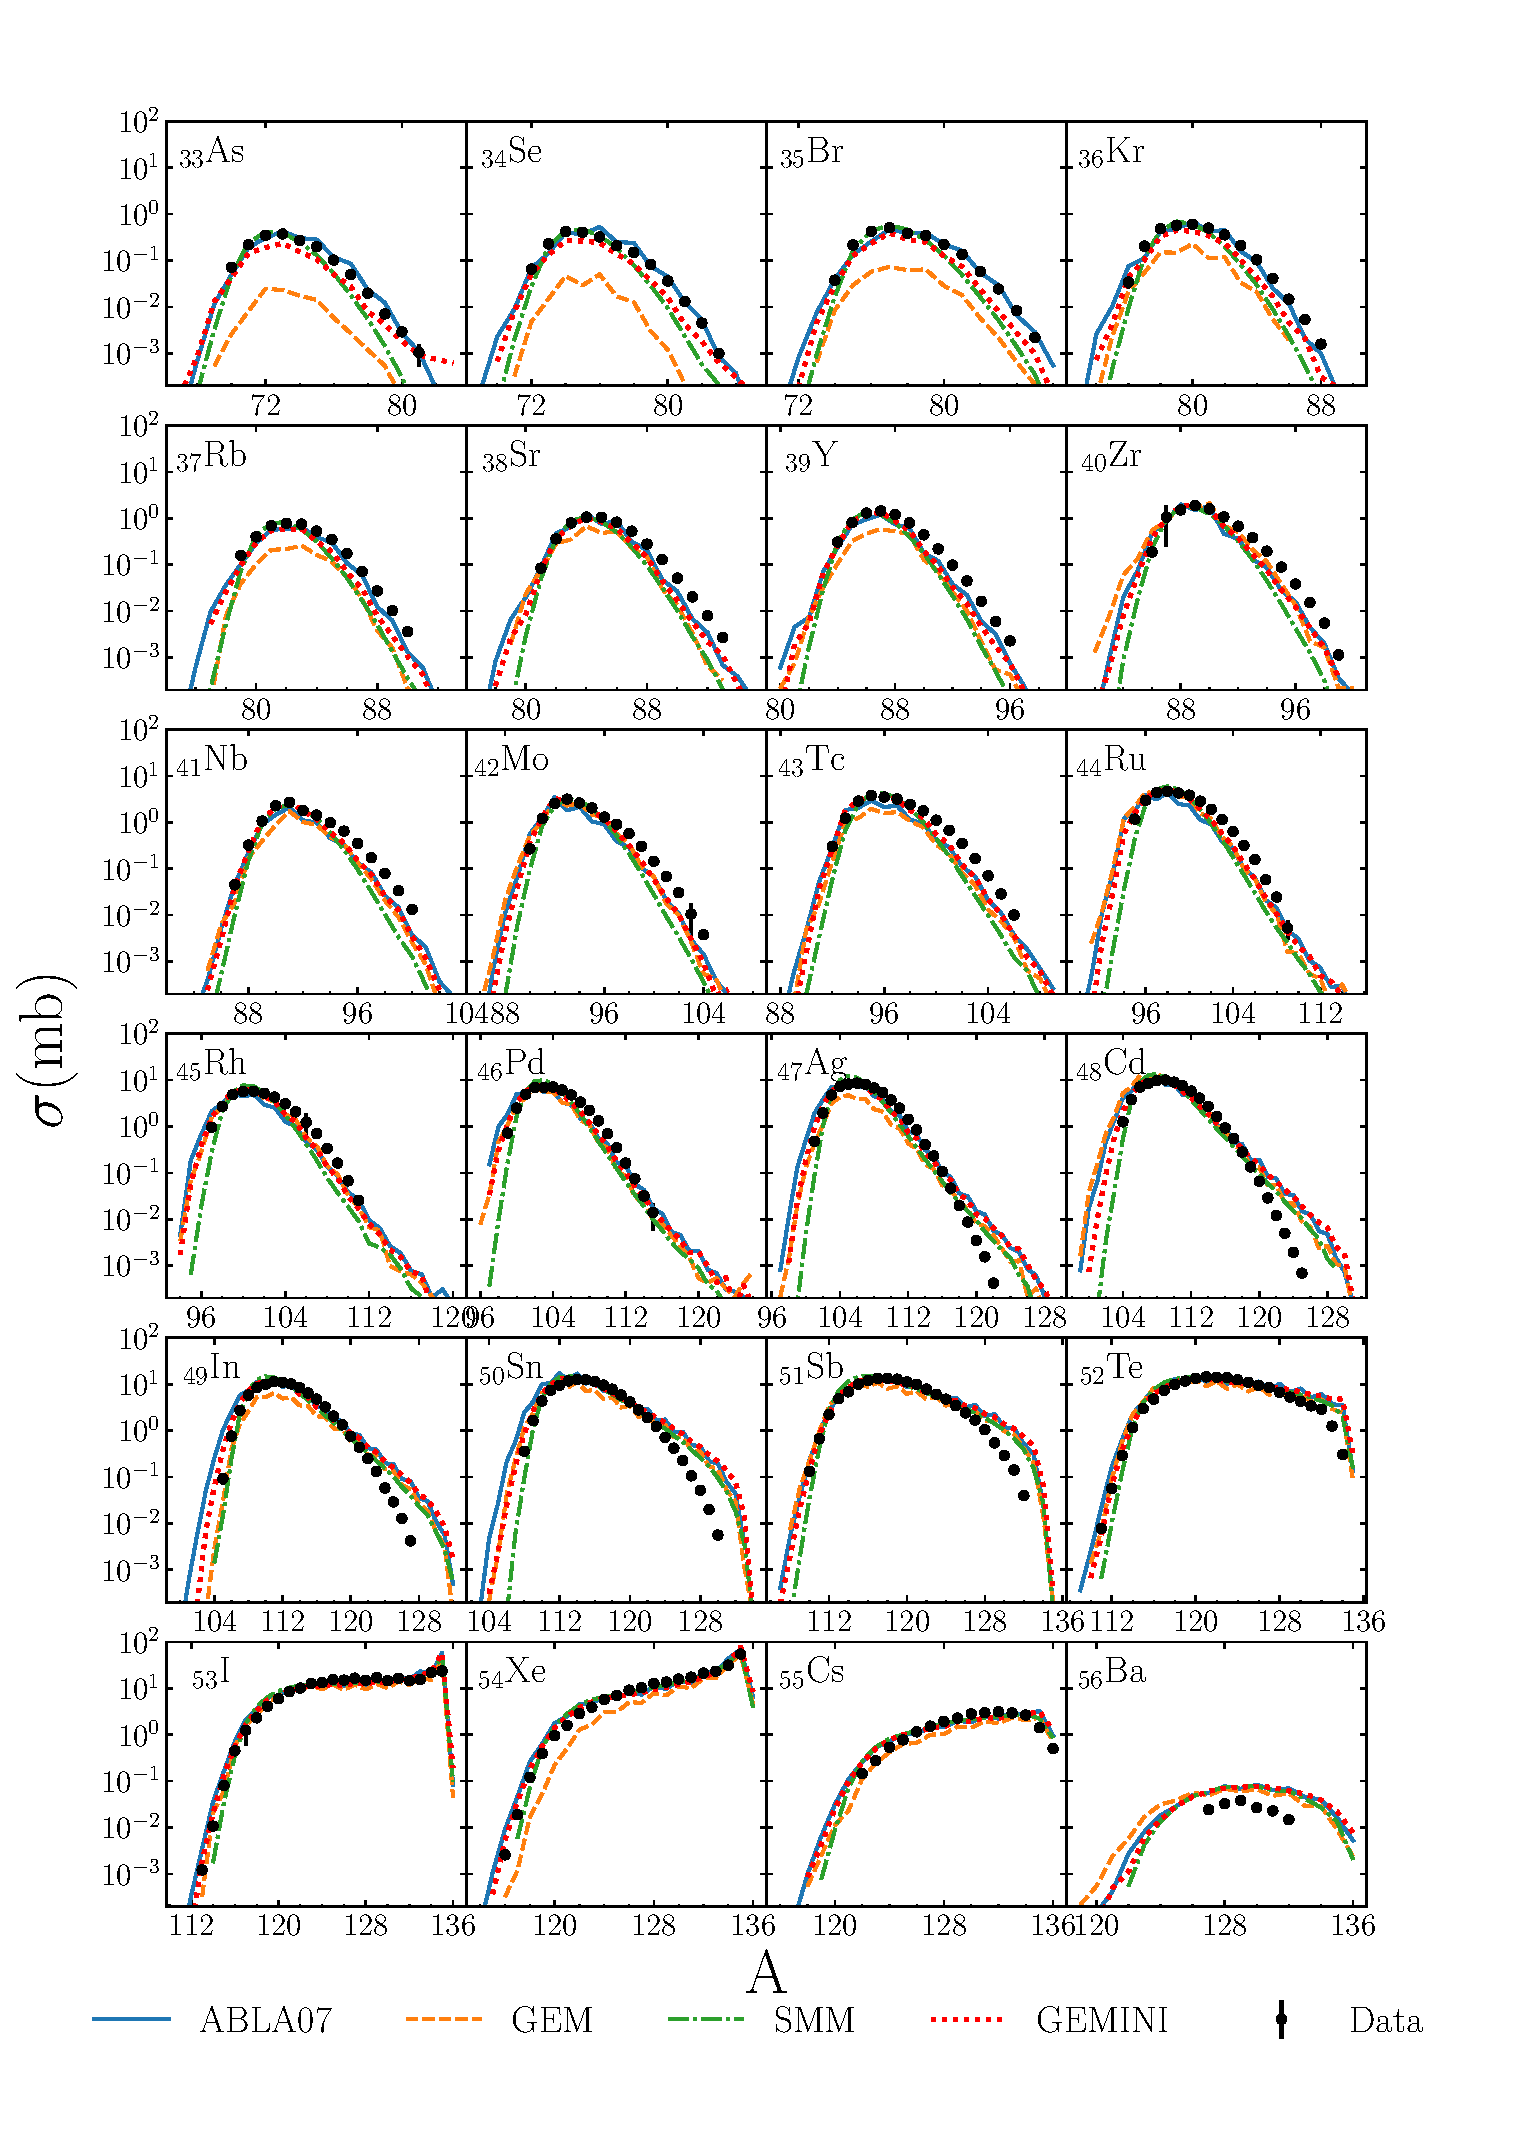
\includegraphics[width=0.95\textwidth]{z3356.eps}
    \caption{The same as in fig. \ref{Z0314}, but for Z = 33–56.}
    \label{Z3356}
\end{figure}

The following qualitative conclusions may be derived from inspection of fig. \ref{Z3356} which presents the isotopic cross-sections measured and calculated for the elements with 32 $<$ Z $<$ 57. The magnitude of the cross-sections predicted by GEM2 model increases with increase of the atomic number of the products. At Z = 33 the model
cross-sections are an order of magnitude smaller than the experimental ones but starting from Z = 40 they start to agree
quite well with the data. The shape of the mass distribution of the isotopic cross-sections predicted by GEM2 for
Z $>$ 40 becomes quite similar to that of the experimental one which is smooth and almost symmetrical up to Z = 47 ($Ac$). 

The other models, i.e., ABLA07, SMM and GEMINI++ reproduce well the shape of the mass dependence
and position of its maximum for all elements starting from Z = 33 ($As$) up to Z = 46 ($Pd$). However, the width of the mass of theoretical and experimental distributions agrees only for ABLA07 and GEMINI++. The SMM model usually
produces too narrow distributions. 

The experimental mass distributions for the range of Z = 47 to Z = 52 of atomic numbers of nuclides (i.e., $Ac$ – $Te$) become asymmetric with the larger values of the cross-sections for the isotopes with large mass number. This behaviour is only partly reproduced by the theoretical models. All of them predict too flat distributions in comparison to the experimental ones. 

As a consequence the values of the experimental cross-sections agree well with the model cross-sections for the lightest isotopes of a given element. They are slightly underestimated for isotopes with average masses and are significantly overestimated (even two orders of magnitude) for the heaviest isotopes. 

The situation changes for reaction products with the largest atomic numbers, i.e., for Z = 53 and Z = 54 ($I$ and $Xe$). In this case the distribution of the isotopic cross-sections monotonically increases with the mass of the  isotopes. All the models reproduce this change of the character of the distributions as well as the magnitude of the cross-sections. The GEM2 model seems to be the poorest in reproduction of $Xe$ (Z = 54) isotopic cross-sections, however it describes well the isotopic cross-sections for $I$ (Z = 53) and $Cs$ (Z = 55). The experimental distribution of the isotopic cross-sections for the element with the largest Z (Z = 56), i.e., for $Ba$, is systematically overestimated by all theoretical models.


\section{Predictive power of the de-excitation models and range of their usage}

The detailed discussion of the agreement between model and experimental isotopic cross-sections presented above does not permit to make a simple, general overview of the quality of description of the data by all examined models. To allow for such an overview the following procedure was applied. 

All isotopes for which the production cross-sections were determined in the experiment \cite{napolitani2007measurement} are presented as empty circles in the two dimensional plot (Z-N) in fig. \ref{ZAfactor}. The isotopes for which the model cross-sections do not deviate more than 10$\%$ from the data are shown as full circles. 

This specific value of the relative deviation was chosen somewhat arbitrary taking into  consideration that the typical relative errors estimated for the most abundant isotopes in the experiment \cite{napolitani2007measurement} are equal to 5$\%$–6$\%$ and do not overcome 20$\%$. 

It may be concluded after inspection of fig. \ref{ZAfactor} that such a representation allows to observe 
characteristic behaviour of the quality of data  reproduction by different models:

\begin{enumerate}[label=\roman*)]
    \item  The number of well described data is rather small. About 12$\%$ of the experimental cross-sections are well reproduced by ABLA07, SMM and GEMINI++ whereas only about 4$\%$ in the case of the GEM2 model.
    
    \item The cross-sections for products with large atomic number Z are more frequently reproduced by the models
    than those for products with small Z. This is especially pronounced in the case of GEM2 where the only reproduced
    experimental cross-sections are those for large Z.

    \item In the case of GEMINI++ several neighbouring isotopes of the same element with the large Z are very well
    reproduced. This is however not the case for other models. It indicates that for these elements GEMINI++ well reproduces
    the shape of the N-dependence of the experimental cross-sections (at least for the largest N values, cf. fig. \ref{Z3356}).
    A quite different situation is present for SMM where two or three lines of well reproduced (Z-N) cross-sections are
    visible. It is caused by the fact that the shape of the mass dependence of isotopic cross-sections predicted by SMM
    is different than the experimental shape. Due to this fact the experimental and theoretical N distributions for given Z
    are crossing at two or three N values (cf. fig. \ref{Z3356}). 

    \item The data for elements with 30 $<$ Z $<$ 40 are not reproduced by GEMINI++ and GEM2 but the ABLA07
    and SMM predictions agree well with the data.

    \item  The data for elements with 20 $<$ Z $<$ 30 are not described by GEM2 and ABLA07 whereas SMM and GEMINI++
    work well for this range of the atomic number.

    \item Isotopic cross-sections for elements with 10 $<$ Z $<$ 20 are not reproduced by GEM2 but some of them are well described by other models.

\end{enumerate}
It is worth emphasizing that different models describe
well different isotopes for this range of atomic number:
GEMINI++ is good for the smallest N-values whereas
ABLA07 and SMM for average N. ABLA07 and 
SMM reproduce well the maximal isotopic  cross-sections 
for given Z. This specific behaviour is caused by the shift 
of the mass distributions produced by ABLA07 and SMM 
towards small N values with respect to the experimental
distributions - cf. fig. \ref{Z0314}.
\begin{figure}
    \centering
    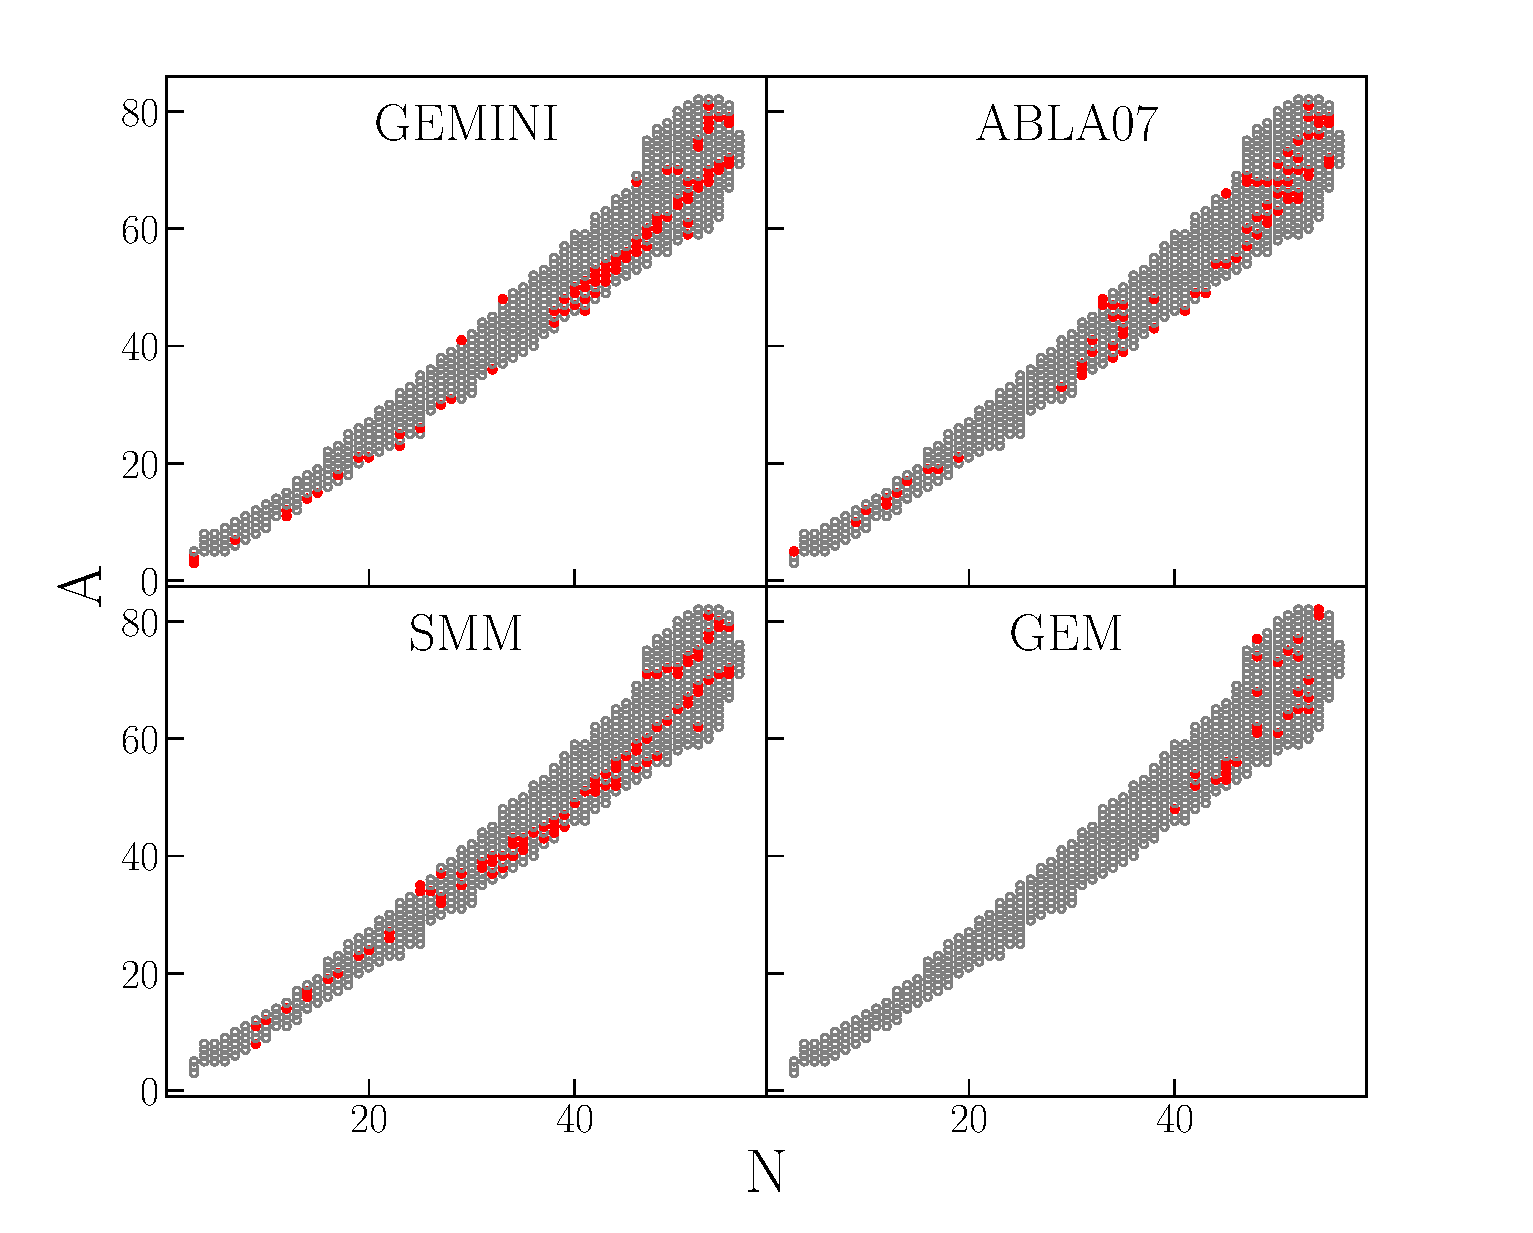
\includegraphics[width=0.85\textwidth]{ZA_Afactorall.eps}
    \caption{The values (Z,N) of experimentally obtained isotopic cross-section in  \cite{napolitani2007measurement} for $^{136}Xe$+$p$ reaction at energy 1 GeV/nucleon (empty circles). The values (Z,N) at which the relative deviation between theoretical ($\sigma^{th}$) and experimental ($\sigma^{exp}$) cross-sections calculated as $2\cdot\left| \sigma^{th}- \sigma^{exp} \right|/(\sigma^{th} + \sigma^{exp})$ is smaller than 10$\%$ are marked with full red circles. The left upper panel contains results of GEMINI++, the right upper panel contains results of ABLA07, the left lower panel contains results of SMM and the right lower panel contains those of GEM2.}
    \label{ZAfactor}
\end{figure}

Another representation of the quality of the model predictions for the isotopic 
cross-sections is application of the $A$-factor (defined in chapter \ref{chapter:4}, formula \ref{A_factor_1}). As it was discussed there  values of the $A$-factor for well predicted 
cross-sections are close to zero. 

The $A$-factor values calculated in this investigation for all the data and for  corresponding combinations of models are presented in fig. \ref{Afactorall}. 

As can be seen in this figure the $A$-factor evaluated
for the GEM2 model cross-sections differs strongly from all others cases. It has values close or equal to one for all
elements with Z between 9 and 30. This is due to the
fact that GEM2 does not produce ejectiles 
in this range of the atomic number Z. 

Other models, which better
reproduce the data provide smaller values of $A$-factor varying between 0.1 and 0.6. 

The following interesting conclusions may be derived from inspection of fig. \ref{Afactorall}:

\begin{figure}
    \centering
    \includegraphics[width=0.9\textwidth]{Afactorall.eps}
    \caption{Values of the $A$-factor evaluated according to equation \ref{A_factor_2}. 
    Blue, open circles represent results obtained for ABLA07, violet open squares correspond to GEM2, green open triangles to SMM whereas yellow solid diamond show values calculated for GEMINI++ results.}
    \label{Afactorall}
\end{figure}
\begin{itemize}
    \item[i)]  The data with 47 $<$ Z $<$ 55 are equally well reproduced
by all the models. This is the range of elements
which are mainly produced by the evaporation of nucleons
from the excited remnant of the intranuclear
cascade.
\item[ii)] For products with 40 $<$ Z $<$ 47 the GEMINI++ model is the best
in reproducing the data. The SMM is the worst 
one in this respect. Results of ABLA07 are randomly better or poorer than those of GEM2.
\item[iii)] The ABLA07 gives distinctly the best description of
the products with 30 $<$ Z $<$ 40. GEMINI++, SMM
and GEM2 lead to the poorer reproduction of the data
with the quality decreasing in the indicated sequence.
\item[iv)] The situation changes for products with 18 $<$ Z $<$ 30
where the GEMINI++ offers the best description of
the data. ABLA07 and SMM compete to provide second
the best reproduction of the experimental cross
sections. The GEM2, which does not produce ejectiles
for this range of atomic number is completely not applicable.
\item[v)] The lowest range of atomic numbers, i.e., Z $<$ 19
seems to be the best described by ABLA07 whereas
GEMINI++ and SMM give comparable, slightly
poorer description.
\end{itemize}
     \begin{longtable}[c]{| c || c |c|c|c|}
     \caption{Ranks of theoretical predictions  of examined in this study models for isotopic distributions
of residua from $Xe$+$p$ collisions at 1 GeV/nucleon \cite{napolitani2007measurement}
according to values of the $A$-factor. For explanation see text. \label{ranktable_long}}\\
     \hline
    \multirow{2}{4em}{Ejectile} &\multicolumn{4}{|c|}{The ranks of the models}\\
    \cline{2-5}
    & ABLA07& GEM2& GEMINI++& SMM\\
    \hline
    \hline
    \endfirsthead
    \hline
 \multicolumn{5}{|c|}{Continuation of Table \ref{ranktable_long}}\\
 \hline
 Ejectile & ABLA07& GEM2& GEMINI++& SMM\\
 \hline
 \hline
    \endhead
\hline
 \endfoot

 \hline
 \hline
Sum of ranks & 116& 195& 91& 138\\
 \hline
  \hline
 Average rank: & 2& 4& 1& 3\\
 \hline
 \endlastfoot
$_{3}$Li & 4 & 3 & 1 & 2 \\
$_{4}$Be & 4 & 3 & 1 & 2 \\
$_{5}$B & 3 & 4 & 2 & 1 \\
$_{6}$C & 1 & 4 & 2 & 3 \\
$_{7}$N & 2 & 4 & 1 & 3 \\
$_{8}$O & 1 & 4 & 3 & 2 \\
$_{9}$F & 1 & 4 & 3 & 2 \\
$_{10}$Ne & 1 & 4 & 2 & 3 \\
$_{11}$Na & 1 & 4 & 2 & 3 \\
$_{12}$Mg & 1 & 4 & 2 & 3 \\
$_{13}$Al & 2 & 4 & 1 & 3 \\
$_{14}$Si & 1 & 4 & 2 & 3 \\
$_{15}$P & 1 & 4 & 2 & 3 \\
$_{16}$S & 1 & 4 & 2 & 3 \\
$_{17}$Cl & 1 & 4 & 2 & 3 \\
$_{18}$Ar & 1 & 4 & 3 & 2 \\
$_{19}$K & 2 & 4 & 1 & 3 \\
$_{20}$Ca & 3 & 4 & 1 & 2 \\
$_{21}$Sc & 3 & 4 & 1 & 2 \\
$_{22}$Ti & 3 & 4 & 1 & 2 \\
$_{23}$V & 2 & 4 & 1 & 3 \\
$_{24}$Cr & 3 & 4 & 1 & 2 \\
$_{25}$Mn & 3 & 4 & 1 & 2 \\
$_{26}$Fe & 3 & 4 & 2 & 1 \\
$_{27}$Co & 3 & 4 & 2 & 1 \\
$_{28}$Ni & 3 & 4 & 1 & 2 \\
$_{29}$Cu & 3 & 4 & 2 & 1 \\
$_{30}$Zn & 3 & 4 & 1 & 2 \\
$_{31}$Ga & 1 & 4 & 3 & 2 \\
$_{32}$Ge & 1 & 4 & 3 & 2 \\
$_{33}$As & 1 & 4 & 2 & 3 \\
$_{34}$Se & 1 & 4 & 2 & 3 \\
$_{35}$Br & 1 & 4 & 2 & 3 \\
$_{36}$Kr & 1 & 4 & 2 & 3 \\
$_{37}$Rb & 1 & 4 & 2 & 3 \\
$_{38}$Sr & 1 & 4 & 2 & 3 \\
$_{39}$Y & 1 & 4 & 2 & 3 \\
$_{40}$Zr & 3 & 2 & 1 & 4 \\
$_{41}$Nb & 2 & 3 & 1 & 4 \\
$_{42}$Mo & 2 & 3 & 1 & 4 \\
$_{43}$Tc & 2 & 4 & 1 & 3 \\
$_{44}$Ru & 3 & 2 & 1 & 4 \\
$_{45}$Rh & 3 & 1 & 2 & 3 \\
$_{46}$Pd & 3 & 2 & 1 & 3 \\
$_{47}$Ag & 1 & 4 & 1 & 3 \\
$_{48}$Cd & 3 & 2 & 1 & 3 \\
$_{49}$In & 3 & 4 & 1 & 1 \\
$_{50}$Sn & 3 & 3 & 2 & 1 \\
$_{51}$Sb & 2 & 4 & 2 & 2 \\
$_{52}$Te & 3 & 3 & 3 & 1 \\
$_{53}$I & 3 & 1 & 3 & 2 \\
$_{54}$Xe & 3 & 4 & 2 & 1 \\
$_{55}$Cs & 2 & 4 & 2 & 1 \\
$_{56}$Ba & 2 & 4 & 2 & 2 \\
\end{longtable}
To summarize this analysis quantitatively, the ranks 
of the models based on values of the $A$-factor were collected
in table \ref{ranktable_long}.
%for all elements produced in the studied here 
%reaction. 
A smaller rank of the model for a given element
means that the model leads to a smaller value of  $A$-factor, thus provides the better description of the data.

If two models give practically the same value of the $A$-factor
then the arithmetic average of their ranks is quoted
in table \ref{ranktable_long} for both models.

The sum of the ranks for a given theoretical 
model for all observed elements can be treated
as a quantitative measure of the quality of its  data description.
%of all the data by the model under consideration.

As can be learn from table \ref{ranktable_long} the quality of the overall 
description of the examined data is the best for GEMINI++ (sum of the ranks is equal to 91). 
The second place in the description of experimental data
is granted to ABLA07 (sum equal to 116). The
third in this respect is SMM (sum equal to 138) and the poorest description of the data is obtained with the use of GEM2 model (sum of ranks equal to 195).

\section{Conclusions about examined second step reaction models}

A very rich set of production cross-sections (over 600) 
%cross-sections) 
measured by Napolitani et al. \cite{napolitani2007measurement} with
isotopic identification of the products for $^{136}Xe$+$p$ collisions
at 1 GeV per nucleon was compared with predictions 
of a two-step reaction scenario simulated with  microscopic theoretical models. 

The first stage of
the reaction was analyzed in the frame of the INCL++
model \cite{INCLboudard2013new}. It treats the proton-nucleus collision as a
sequence of nucleon-nucleon and nucleon-pion collisions
leaving the equilibrated, excited remnant nucleus. 

The description of the second
stage of the reaction was tested with the use 
of four different models: ABLA07  \cite{kelic2009abla07}, GEM2  \cite{FURIHATA2000,Furihata2002}, GEMINI++ \cite{CHARITY1988,Charity2010} 
and SMM \cite{SMMBondorf1995}. They assume different scenarios of the
de-excitation process of the intranuclear 
cascade remnant.

All calculations were performed using the default values
of the applied theoretical models with the aim to study
the predictive power of the models in respect to the determination
of isotopic cross-sections.

It was found that ABLA07, SMM and GEMINI++ reproduce
the main properties of the Z and A dependence of the cross-sections for reaction products which cover very
broad range of elements (from $_{3}Li$ to $_{56}Ba$) whereas the
GEM2 gives comparably good predictions only for lithium
and for the elements with large atomic number (Z $>$ 40).

This is illustrated by figs. \ref{Z0314}, \ref{Z1532} and \ref{Z3356}, which present the data and
the theoretical cross-sections for separate ranges of atomic
number Z of the products. Inspection of these figures allows
to estimate qualitatively the agreement between the 
data and the model predictions.

A very good quantitative reproduction of the experimental
isotopic cross-sections, i.e., such which results in
the relative deviation between the data and the model
cross-sections smaller than 10\%, was achieved only for a
small part of all the cross-sections as it is shown in fig. \ref{ZAfactor}.

The models ABLA07, SMM and GEMINI++ offer such a
perfect reproduction of data for approximately 12\% of the
products whereas GEM2 only for approximately 4\%. This
suggests that the models under consideration cannot be
approved if the main criterion would be the  perfectness of the cross-sections prediction 
for isotopically resolved reaction products.

Better but also not perfect prediction of the cross-sections
was found when the average agreement over isotopes
of given element is considered. Such a quantitative comparison
of the model and experimental cross-sections was
achieved by the application of the $A$-factor  which was described in chapter \ref{chapter:4}. 

%a reference \cite{sharma2017ranking}  
%dealing with the reactions in the same nuclear system,
%i.e., $^{136}Xe$ + p but at twice smaller energy (500MeV per nucleon). 

The Z-dependence of the $A$-factor presented in
fig. \ref{Afactorall} shows that the production cross-sections of elements
with largest atomic numbers are equally well reproduced
by all applied models. The situation changes for
smaller atomic numbers. Then the different models assure the
best description for different ranges of the atomic number
of products. 

The ranking of models based on achieved values
of the $A$-factor was made (cf. table \ref{ranktable_long}) which clearly
shows that the averaged over isotopes and elements agreement
between the data and experimental cross-sections is
the best for GEMINI++. 
The ABLA07 and SMM produced
poorer average agreement and the GEM2 is the
worst.

These conclusions agree with result obtained in the work \cite{sharma2017ranking} in which the analysis of the data measured 
at lower energy, i.e., 500 MeV per nucleon for the
same nuclear system were investigated. 
But then only elements with Z $>$ 40 were studied. 

%The data were reproduced
%in the best way by GEMINI++, however the SMM
%model gave better description than ABLA07 whereas
%GEM2 also achieved the last position. The conclusion that
%the values of the $A$-factor are too big to claim that the
%studied models may be approved remains true also after the present analysis.
